% Section content template for individual Educative lessons
% This file contains the actual content for a specific section
% Generated from Educative API section content

% Section: Use Case Diagram for Stack Overflow
% Section ID: 4790351711961088
% Section Slug: use-case-diagram-for-stack-overflow
% Generated: 2025-12-12T22:49:13.721000

Let's build the Stack Overflow use case diagram and understand its components' relationship. First , we'll define the different elements of our Stack Overflow system, followed by the complete use case diagram.

\subsection{System}\label{vbJ8VWG2gx0eUXyggdhvB}
\\
Our system is Stack Overflow.

\subsection{Actors}\label{SJq1WEROQkxai3INR_Hc4}
\\
Now, we'll define the main actors of Stack Overflow.

\subsubsection{Primary actors}\label{m9EG8iuRfRtsaPDo__W8d}

\begin{itemize}
\item
\textbf{User:} A registered user who can

\begin{itemize}
\item
Create, edit, and flag questions and answers.
\item
Add bounties and tags.
\item
Upvote/downvote content.
\item
Accept answers.
\item
Add comments.
\item
Vote to close/delete questions and answers.
\end{itemize}
\item
\textbf{Moderator:} A privileged user who can

\begin{itemize}
\item
Close, delete, reopen, and restore questions.
\item
Delete answers.
\end{itemize}
\end{itemize}

\subsubsection{Secondary actors}\label{QdKhmIgRSSztFD_hb0qvS}

\begin{itemize}
\item
\textbf{Guest:} An unregistered visitor who can

\begin{itemize}
\item
Search for and view questions and answers.
\item
Register an account.
\end{itemize}
\item
\textbf{Admin:} A system administrator who can

\begin{itemize}
\item
Block or unblock users.
\item
Award badges manually.
\end{itemize}
\item
\textbf{System:} Responsible for

\begin{itemize}
\item
Awarding badges based on rules.
\item
Sending notifications (on answer, comment, or vote).
\end{itemize}
\end{itemize}

\subsection{Use cases}\label{hbN7X8Ukq4zCeFkaBe5Om}
\\
In this section, we'll define the use cases for Stack Overflow and list them according to their interactions with a particular actor.
\begin{quote}
\textbf{Note:} Some use cases will occur multiple times because they are shared among different actors in the system.
\end{quote}
\subsubsection{User}\label{okJUJF6rHqL3DacFw4oeK}

\begin{itemize}
\item
\textbf{Add/Modify/Flag Question:} Toallow users to post new, update, or report inappropriate questions.
\item
\protect\phantomsection\label{dCiMA08R_jQRNPEjKs0KX}
\textbf{Add/Modify/Flag Answer:} Toenable users to contribute answers, edit content, or flag problematic responses.
\item
\protect\phantomsection\label{IA7xR9tycCBMO8CHOgAJL}
\textbf{Add Comment:} To let users add clarifying or supporting comments on questions and answers.
\item
\protect\phantomsection\label{A2OFxLl34jUloElEhhmCI}
\textbf{Upvote a Comment:} To empower users to upvote a comment.
\item
\protect\phantomsection\label{f2v4lp3_BXpBJCeobqGb6}
\textbf{Add Bounty:} To let users offer reputation points to attract answers to their questions.
\item
\protect\phantomsection\label{bL6dW7F6HTQDCFxSpemy9}
\textbf{Add Tag:} To let users label questions with relevant topic tags for better discoverability.
\item
\protect\phantomsection\label{BFVUkToCOSK7xCJchBhNQ}
\textbf{Vote to Close / Delete Question:} To empower users to initiate closure or deletion of low-quality or off-topic questions.
\item
\protect\phantomsection\label{Wp_j3PTfG5Qqkfp8-U2TR}
\textbf{Vote to Delete Answer:} To empower users to initiate the deletion of low-quality answers.
\item
\protect\phantomsection\label{7abTA_lHwQQr18s9PUqDL}
\textbf{Upvote / Downvote to Question / Answer:} To enable users to express approval or disapproval of questions and answers.
\item
\protect\phantomsection\label{Dn5LL8C-0dhFxwm918ndY}
\textbf{Accept Answer:} To let the authors mark the most helpful answer as accepted.
\end{itemize}

\subsubsection{Guest}\label{UmThuzJ318y8Gg0HlkKZA}

\begin{itemize}
\item
\protect\phantomsection\label{6TteFajqIJ7PkaUv-csSd}
\textbf{Search / View Question:} To allow non-logged-in users to browse and search for public questions and answers.
\item
\protect\phantomsection\label{mZ5zmcHjl5dRYITFp8yQ-}
\textbf{Register Account:} To enable guests to sign up and become a full-featured user.
\end{itemize}

\subsubsection{Admin}\label{c-EjaMXHWXMYpN7pbMGn4}

\begin{itemize}
\item
\protect\phantomsection\label{U0ElkZkzKBMP6N7y4vbxW}
\textbf{Block / Unblock User:} To enable administrators to restrict or restore user access to the platform.
\item
\protect\phantomsection\label{b0D9Dx6jZfpaJO24Get15}
\textbf{Award Badge:} To allow admins to assign special badges manually to recognize user contributions.
\end{itemize}

\subsubsection{Moderator}\label{h4ESnO7fkn46xMWJg1wPN}

\begin{itemize}
\item
\protect\phantomsection\label{db5ui158FSKbEMuKoZ6Af}
\textbf{Close / Reopen / Delete / Restore Question:} To grant moderators authority to manage question visibility and status.
\item
\protect\phantomsection\label{ENZEomqRoxDP4CHLtfD1o}
\textbf{Delete Answer:} To allow moderators to permanently remove inappropriate or low-quality answers.
\end{itemize}

\subsubsection{System}\label{a5Q-HeDaKYUz6lbpB96PB}

\begin{itemize}
\item
\protect\phantomsection\label{JQ9sptSON0dMuLknILv7z}
\textbf{Send Notification:} To automatically inform users of interactions like votes, comments, answers, or badges.
\item
\protect\phantomsection\label{WGWba8uaIqxgotOHhJmOx}
\textbf{Award Badge:} To automatically grant achievement badges based on predefined contribution criteria.
\item
\protect\phantomsection\label{WNtDiUngTfZ0hP7P0-G-0}
\textbf{Determine Popular Tags:} To automatically determine the most popular tags.
\end{itemize}

\subsection{Relationships}\label{ZLLCJL3zC0JhX2cfP-5x8}
\\
This section describes the relationships between and among actors and their use cases.

\subsubsection{Generalization}\label{KxP_kk2X6_r43zzvw7gjQ}

\begin{itemize}
\item
\protect\phantomsection\label{1Tz-fI0zxJrElpolMV5nT}
``Moderator'' has a generalization relationship with ``User'' as the moderator can perform all the tasks a normal user can perform.
\item
\protect\phantomsection\label{UIbDjBkPHmctUJH495qtX}
``User'' has a generalization relationship with ``Guest'' as the normal user can perform all those tasks that a guest user can perform.
\end{itemize}

\subsubsection{Associations}\label{sC7xa3eLcACG2l7_CgVN7}
\\
The table below shows the association relationship between actors and their use cases.

\begin{table}[htbp]
\centering
\small
\adjustbox{max width=\textwidth}{
\begin{tabular}{|p{0.208\textwidth}|p{0.179\textwidth}|p{0.147\textwidth}|p{0.258\textwidth}|p{0.158\textwidth}|}
\hline
\textbf{User} & \textbf{Guest} & \textbf{Admin} & \textbf{Moderator} & \textbf{System} \\
\hline
\hline
Search/view question & Register account & Block/unblock user & Search/view question & Award badge to user \\
\hline
Vote to close/delete question & Search/view question & Award badge & Vote to close/delete question & Send notification \\
\hline
Accept answer & \hfill\break & \hfill\break & Accept answer & Determine popular tags \\
\hline
Add/modify/flag question & \hfill\break & \hfill\break & Add/modify/flag question & \hfill\break \\
\hline
Add/modify/flag answer & \hfill\break & \hfill\break & Add/modify/flag answer & \hfill\break \\
\hline
Add comment & \hfill\break & \hfill\break & Add comment & \hfill\break \\
\hline
Upvote/downvote question/answer & \hfill\break & \hfill\break & Upvote/downvote question/answer & \hfill\break \\
\hline
Upvote a comment & \hfill\break & \hfill\break & Close/reopen/delete/restore question & \hfill\break \\
\hline
Vote to delete answer & \hfill\break & \hfill\break & Delete answer & \hfill\break \\
\hline
\hfill\break & \hfill\break & \hfill\break & Upvote a comment & \hfill\break \\
\hline
\hfill\break & \hfill\break & \hfill\break & Vote to delete answer & \hfill\break \\
\hline
\end{tabular}
}
\end{table}

\subsubsection{Include}\label{E6c3ykAkGs3AZ07d6dOGz}
\\
A notification is triggered when a user interacts with content, such as adding an answer or comment, voting, accepting an answer, awarding a badge, or posting a new question.

\begin{itemize}
\item
The ``Send a notification'' use case includes the ``Add an answer,'' ``Add a comment,'' ``Upvote/Downvote a question/answer,'' ``Accept an answer,'' ``Award a badge,'' ``Upvote a comment,'' and ``Add a question'' use cases.
\end{itemize}
\\
Users can assign a bounty or add tags when posting a new question.

\begin{itemize}
\item
The ``Add a question'' use case includes the ``Add bounty'' and ``Add a tag'' use cases.
\end{itemize}
\\
When a user modifies a question, they may also update its bounty or tags.

\begin{itemize}
\item
The ``Modify a question'' use case includes the ``Add bounty,'' ``Add a tag,'' ``Modify bounty,'' and ``Modify the tag'' use cases.
\end{itemize}

\subsection{Use case diagram}\label{ntuDu8WMaZWZ75w_L5Zjh}
\\
Here's the use case diagram of Stack Overflow:

\begin{figure}[htbp]
 \centering
 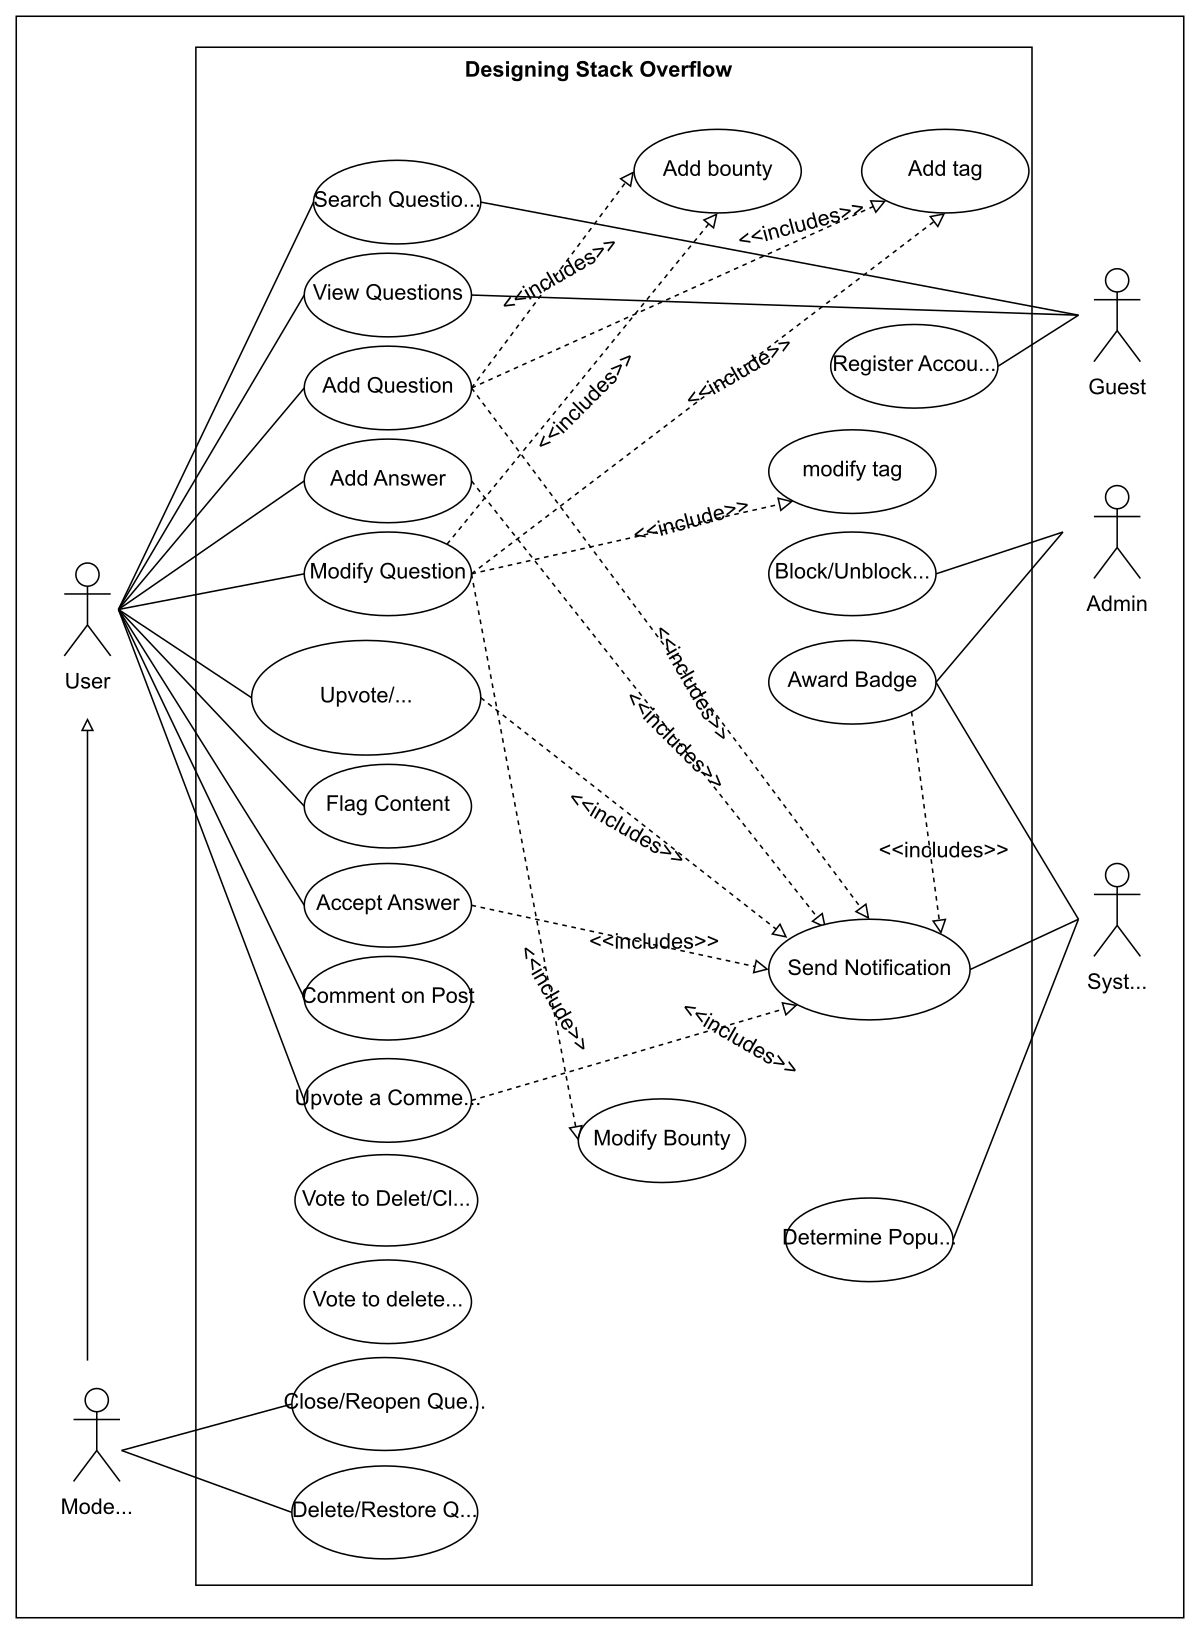
\includegraphics[width=0.5\textwidth]{Images/chapter_20/section_4790351711961088/6245092187570176.png}
 \caption{The use case diagram for Stack Overflow}
\end{figure}

\hfill\break
In the next lesson, we will discuss the class diagram with a detailed explanation of all classes and their relationship with each other.

% End of section content